\documentclass[twoside,11pt]{article}


% Any additional packages needed should be included after jmlr2e.
% Note that jmlr2e.sty includes epsfig, amssymb, natbib and graphicx,
% and defines many common macros, such as 'proof' and 'example'.
%
% It also sets the bibliographystyle to plainnat; for more information on
% natbib citation styles, see the natbib documentation, a copy of which
% is archived at http://www.jmlr.org/format/natbib.pdf

% Available options for package jmlr2e are:
%
%   - abbrvbib : use abbrvnat for the bibliography style
%   - nohyperref : do not load the hyperref package
%   - preprint : remove JMLR specific information from the template,
%         useful for example for posting to preprint servers.
%fhajkfhcuhfkahficdaui
% Example of using the package with custom options:
%
% \usepackage[abbrvbib, preprint]{jmlr2e}

\usepackage[preprint]{jmlr2e}
\usepackage{array}
\usepackage{longtable}
\usepackage{booktabs}

\ShortHeadings{Novel Approach to deal with Data Imbalance in Automobile Insurance Fraud Data}{Alshamsi, Farhan and Mohammed}
\firstpageno{1}

\begin{document}

\title{Novel Approach to deal with Data Imbalance in Automobile Insurance Fraud Data}

\author{\name Abdus Saboor Gaffari Mohammed \email b00105302@aus.edu \\
        \addr Department of Computer Science \& Engineering\\
        Master of Science in Machine Learning\\
        American University of Sharjah\\
        Sharjah, UAE
        \AND
        \name Alizar Farhan \email @aus.edu \\
        \addr Department of Computer Science \& Engineering\\
        Master of Science in Computer Engineering\\
        American University of Sharjah\\
        Sharjah, UAE
        \AND
        \name Khalifa Alshamsi \email b00078654@aus.edu \\
        \addr Department of Computer Science \& Engineering\\
        Master of Science in Machine Learning\\
        American University of Sharjah\\
        Sharjah, UAE
       } 

\maketitle

\begin{abstract}%   <- trailing '%' for backward compatibility of .sty file
Abstract
\end{abstract}

\begin{keywords}
  keyword one, keyword two, keyword three
\end{keywords}

\section{Introduction}
The insurance sector is one of the oldest and largest financial sectors, providing financial protection from losses to individuals. Insurance is an agreement between an insurer and insured party (policyholder), in which the insurer promises financial compensation to the insured party in cases of an accident or specific loss (\citealp{viaeneInsuranceFraudIssues2004}), given that the insured party has placed a claim. This process of claiming financial compensation poses as an opportunity for malicious actors, who place false claims. These fraudulent claims are referred to as insurance fraud. One of the areas of insurance sector that is particularly vulnerable to frauds is the automobile insurance.

Automobile insurance fraud is a growing concern for the insurance industry as it significantly affects both the insurers and policyholders. Fraudulent activities can be in various forms like, over-inflated damage claims involving excessive repair costs, staged accidents including preplanned collisions involving one or more parties, and report fraudulent injuries to exploit medical coverage benefits. As these frauds go undetected, they increase the cost that is incurred to the insurance companies, who inturn increase the premiums of policies they provide, which ultimately leads to the honest customers in paying more for their policies. According to a report by Forbes (\citealp{kilroyInsuranceFraudStatistics2024}), insurance frauds imposed severe economic consequences, with an estimated annual cost of \$308.6 billion to the U.S. economy. This increased financial burden and cost for insurance companies is ultimately passed on to honest policyholders, who face increased premiums ranging between \$400 and \$700 annually per household.

In order to detect these activities in earlier times, insurance companies have sought out to investigating the claims by traditional methods. But these traditional methods rely on manual reviews and rule-based systems, which are time consuming, costly and prone to human error. The also introduces unwarrented scrutiny of legitimate claims (\citealp{AndreasRp,BERMUDEZ}). To tackle with these issues, experts have come up with many statistical models to detect insurance frauds like the one presented by \citealp{belhadjiModelDetectionInsurance2000}, which are still lag in performace and effeciency. 

The advent of machine learning (ML) and artificial intelligence (AI) has introduced transformative approaches to fraud detection. By leveraging advanced techniques such as anomaly detection, predictive modeling, and behavior analysis, insurers can identify patterns indicative of fraud. However, these methods face a significant challenge: data imbalance. Fraudulent claims typically represent a small fraction of the total dataset, leading models to focus disproportionately on the majority class (genuine claims). This imbalance reduces the model's sensitivity to fraudulent cases, resulting in poor detection rates and overfitting problems (\citealp{phuaComprehensiveSurveyData2012}). Additionally, the lack of publicly available high-quality datasets, due privacy concerns, further complicates efforts to improve fraud detection systems, as researchers often struggle with insufficient or skewed data.

\subsection{Contribution and Plan}

As we have already discussed, the main issues that pertain to automobile insurance fraud detection using machine learning is the unavailability of data and the imbalance of fraud and non-fraud cases within the data. These issues forms the basis of our reasearh question:

\begin{itemize}
    \item How can we improve the performance of existing machine learning techniques?
    \item How can we deal with the issue of data imbalance?
\end{itemize}

To address both these questions, we plan to use synthetic data generated using TVAE (\citealp{XuRp}). To tackle the first question we generated synthetic records for both the classes using TVAE and augmented them to the original data, effectively increasing the size of the datset. By creating more synthetic samples in the training data we aim to help make the model more robust and better generalizable to the unseen test data.

To tackle the second question, we used the TVAE again, but in this case we only generated synthetic data for the minority class, making sure that we only generate just enough samples that the number of fraud and non-fraud cases become equal. Using these two approaches, we plan to prove how TVAE can be used for effeciently balance the data and achieve better performance at the same time using oversampled synthetic data. Finally, for the classification task, we plan to use ensemble decision tree models like XGBoost and Random forest, which have proven to work well the the datset we have chosen.

To summarize, this study focuses on addressing the issue of data imbalance in automobile insurance fraud detection while improving the performance of machine learning techniques. Specifically, it explores the generation of synthetic datasets, the application of advanced ML models, and the challenges posed by limited data availability. The research aims to contribute to the development of robust and efficient fraud detection frameworks that not only mitigate the economic impact of fraud but also enhance the experience of genuine policyholders.

The rest of the paper is organized in the following manner, Section \ref{sec:background} will introduce to some key concepts that the paper deals with followed by Section \ref{sec:relatedwork} talking about some of the related works in the same domain and their challenges. Section \ref{sec:method} will introduce to the chosen datset, the proposed methodology, and data preprocessing techniques employed. This is followed by the details on evaluation method used, results and discussions on the results in Section \ref{sec:result}. Finally Section \ref{sec:conclusion} will provide the conclusions and future directions.

\section{Background} \label{sec:background}
\subsection{Data Imbalance}
Data Imbalance refers to a situation in machine learning and data analysis where the distribution of classes in a dataset is highly uneven, with one class significantly outnumbering the other(s). This is common in real-world scenarios such as fraud detection, medical diagnosis, and anomaly detection, where the minority class (e.g., fraudulent claims, rare diseases) is often the most critical but underrepresented. Data imbalance poses challenges for machine learning models, as they tend to favor the majority class, leading to poor performance in predicting the minority class.
To address this, techniques such as oversampling (e.g., SMOTE \citealp{chawlaSMOTESyntheticMinority2002}) or undersampling can be employed. Additionally, cost-sensitive learning and ensemble methods are also effective in enhancing the model's focus on minority class predictions (\citealp{garcia2009}). Proper evaluation metrics like F1-score, precision-recall curves, and area under the precision-recall curve (AUC-PR) are essential for assessing performance on imbalanced datasets (\citealp{fernandezPerformanceMeasures2018a}).
By addressing data imbalance, models can better generalize and improve performance in critical applications, ensuring fairness and reliability in decision-making tasks.

\subsection{Data Leakage}
Data leakage in machine learning occurs when the attributes and features of the test data are introduced in the training data, and these attributes or features won't be availabe during the actual prediction stage of the model. Data leakage lead to having a good or excellent peroformance in the training and testing phase, but fails in the production phase. The common causes of data leakage include improper preprocessing, flawed feature engineering, or cross-validation errors \cite{Kaufman2012}. Data leakage can also be a result of oversampling the data before the data is split for training. When the data is split into train and test after oversampling, the data samples that are very similar, or identical in some cases, to the test data are introduced in the training data which leads the model to overfit to the test resulting in good testing performance. Data leakage is of more concern in the cases like fraud and fault identification as these involve detectuion of anomalies and outliers. Data leakage in these cases causes the model to memorize the fraudulent data rather than understanding the underlying patterns (\citealp{baesensRobROSERobustApproach2021}).

\subsection{Synthetic Data}
Synthetic Data refers to artificially generated data that imitates actual-world information at the same time as keeping its statistical and structural format. According to \citealp{SyntheticPatki2016}, synthetic data may be created by the usage of algorithms, simulations, or generative models like GANs (Generative Adversarial Networks) and is used when real information is inaccessible, constrained, or sensitive.
In simple terms, synthetic data acts alternatively for real records. For example, in training gadget learning models, synthetic data allows builders to test their algorithms without exposing non-public or private information. due to privacy constraints, It is typically utilized in fields like healthcare, finance, and autonomous structures to stability privacy, price, and scalability while ensuring information diversity and application.

\section{Related Works}\label{sec:relatedwork}



\begin{longtable}{>{\hspace{0pt}}m{0.198\linewidth}>{\hspace{0pt}}m{0.096\linewidth}>{\hspace{0pt}}m{0.306\linewidth}>{\hspace{0pt}}m{0.337\linewidth}}
\caption{}
\label{tbl:relatedworks}\\
\toprule
\centering
\textbf{Work}                                          & \textbf{Balance Technique} & \textbf{Strengths}                                                                           & \textbf{Weaknesses}                                                                                    \endfirsthead
\citealp{Patel2019}                                    & FCM + SMOTE                & Under sampling via removing outliers + Generate synthetic samples to balance datasets                   & High computational cost due to clustering. Can introduce noise or synthetic data artifacts, leading to overfitting.  \\
\citealp{Salmi2022,Patel2019}                          & Random oversampling        & Easy to construct                                                                                       & Can lead to overfitting by duplicating existing data                                                                 \\
\citealp{Salmi2022,Patel2019}                          & Random undersampling       & Easy to construct, reduces computational cost                                                           & Can lead to loss of valuable information from the majority class                                                     \\
\citealp{Patel2019,Harjai2019,Salmi2022,Wongpanti2024} & SMOTE                      & Generate synthetic samples to balance datasets, widely used                                             & Can introduce noise or synthetic data artifacts, leading to overfitting                                              \\
\citealp{Salmi2022}                                    & ROSE                       & Generates more diverse synthetic samples                                                                & Computationally intensive and may add noise to the dataset                                                           \\
\citealp{Wongpanti2024}                                & ADASYN                     & Generate synthetic samples for harder-to-classify instances                                             & May skew data distribution, leading to overfitting in some cases                                                     \\
\citealp{Wongpanti2024}                                & GAN                        & Generates realistic synthetic data by mimicking data distribution                                       & Requires extensive training and is computationally expensive                                                         \\
\citealp{Wongpanti2024}                                & CTGAN                      & Generates realistic synthetic data by mimicking data distribution, effectively handles categorical data & More complex and computationally intensive than GAN                                                                  \\
\bottomrule
\end{longtable}

\section{Methodology} \label{sec:method}


\subsection{Dataset}
The dataset used in this research is the \emph{carclaims.txt} data that was originally made available as part of the Agnoss Knowledge Seeker product. The original copy of the data is no longer available for download, but many publicly available copies are available through GitHub\footnote{https://github.com/Rashmi-77/Vehicle-Insurance-Fraud-Detection} and Kaggle\footnote{https://www.kaggle.com/datasets/khusheekapoor/vehicle-insurance-fraud-detection}. The dataset contains 15,420 samples of automobile insurance claims from an insurance company for the years from 1994 to 1996. Out of the 15,420, only 923 are fraudulent claims indicating a very high imbalance in the date. This particular dataset was chosen because there are not many publicly available datasets on automobile insurance fraud, and the ones that are available are very small. Another reason for choosing this data is that this has been extensively used in many other research on automobile insurance fraud detection (\citealp{schrijverAutomobileInsuranceFraud2024, Salmi2022, Padhi2020, Wongpanti2024, Harjai2019, Patel2019}), making it easy for comparative analysis.

Table \ref{tab:dataCols} shows the various columns of the data and their details. Out of 33 columns only two columns are numerical, Age and PolicyNumber, and the remaining columns are all categorical including the target feature FraudFound. The main drawbacks of this data is that due to its small size and high imbalance the model performances is usually low, leading researches to employ oversampling techniques.

\begin{longtable}{>{\hspace{0pt}}m{0.202\linewidth}>{\hspace{0pt}}m{0.414\linewidth}>{\hspace{0pt}}m{0.16\linewidth}>{\hspace{0pt}}m{0.11\linewidth}} 
\caption{Details about the columns of the dataset - \emph{carclaims.txt}}
\label{tab:dataCols}\\
\toprule
\textbf{Column}      & \textbf{Description}                                                                                        & \textbf{Type}  & \textbf{Subtype}  \endfirsthead
PolicyNumber         & Unique identifier for the policy                                                                            & Numerical (PK) & Discrete          \\
Month                & Month when the incident occurred                                                                            & Categorical    & Ordinal           \\
WeekOfMonth          & Week of the month when the incident occurred                                                                & Categorical    & Ordinal           \\
DayOfWeek            & Day of the week when the incident occurred                                                                  & Categorical    & Ordinal           \\
Make                 & Make of the vehicle involved in the incident                                                                & Categorical    & Nominal           \\
AccidentArea         & Area where the accident occurred (Urban or Rural)                                                           & Categorical    & Nominal           \\
DayOfWeekClaimed     & Day of the week when the claim was made                                                                     & Categorical    & Nominal           \\
MonthClaimed         & Month when the claim was made                                                                               & Categorical    & Nominal           \\
WeekOfMonthClaimed   & Week of the month when the claim was made                                                                   & Categorical    & Nominal           \\
Sex                  & Gender of the policyholder                                                                                  & Categorical    & Nominal           \\
MaritalStatus        & Marital status of the policyholder                                                                          & Categorical    & Nominal           \\
Age                  & Age of the policyholder (or) policy \footnote{This is not made clear in the data or any supporting sources} & Numerical      & Discrete          \\
Fault                & Indicates fault (Policy Holder or Third Party)                                                              & Categorical    & Nominal           \\
PolicyType           & Type of insurance policy                                                                                    & Categorical    & Nominal           \\
VehicleCategory      & Category of the vehicle (e.g., Sport, Utility, Sedan)                                                       & Categorical    & Nominal           \\
VehiclePrice         & Price range of the vehicle                                                                                  & Categorical    & Ordinal           \\
RepNumber            & Identifier for the representative managing the case                                                         & Numerical      & Discrete          \\
Deductible           & Deductible amount in the policy                                                                             & Categorical    & Ordinal           \\
DriverRating         & Driver rating (1 to 4)                                                                                      & Categorical    & Nominal           \\
Days:Policy-Accident & Days between policy start and accident                                                                      & Categorical    & Ordinal           \\
Days:Policy-Claim    & Days between policy start and claim                                                                         & Categorical    & Ordinal           \\
PastNumberOfClaims   & Number of claims made in the past                                                                           & Categorical    & Ordinal           \\
AgeOfVehicle         & Age of the vehicle involved in the incident                                                                 & Categorical    & Ordinal           \\
AgeOfPolicyHolder    & Age range of the policyholder                                                                               & Categorical    & Ordinal           \\
PoliceReportFiled    & Indicates if a police report was filed (Yes/No)                                                             & Categorical    & Nominal           \\
WitnessPresent       & Indicates if a witness was present (Yes/No)                                                                 & Categorical    & Nominal           \\
AgentType            & Type of agent (Internal or External)                                                                        & Categorical    & Nominal           \\
NumberOfSuppliments  & Number of claim supplements                                                                                 & Categorical    & Ordinal           \\
AddressChange-Claim  & Time since the last address change                                                                          & Categorical    & Ordinal           \\
NumberOfCars         & Number of cars in the policy                                                                                & Categorical    & Ordinal           \\
Year                 & Year of the incident                                                                                        & Categorical    & Nominal           \\
BasePolicy           & Basic policy coverage (e.g., Liability, Collision)                                                          & Categorical    & Nominal           \\
FraudFound           & Indicates if fraud was found in the claim                                                                   & Categorical    & Nominal           \\
\bottomrule
\end{longtable}


\subsection{Proposed Approach}
The proposed model to balance the automobile insurance fraud data and to improve the performance of the ML models, uses a TVAE to generate synthetic data to balance the data and generate additinal samples for training the ML models. As shown in Figure \ref{fig:model} in the first phase of training, after the dataset is split into train and test set, the train set is used to train the TVAE. After the TVAE is trained, it is used to generate synthetic data that resembels the distributions of the original training data. The number of samples generated for each of the classes is determined by the imbalance between the classes and a predefined value that dictates the number of additional samples to be generated for both the classes. 

First the difference in the number of occurences of the minority and majority classes is calculated. This difference is then added to the predefined value, this resulting value is used as the number of synthetic samples to be generated for the minority class using TVAE. Finally, the unchanged predefined value is used as the number of synthetic samples to be generated for the majority class. Combining these samples with the original trai set gives us a balanced and oversampled training data that can be used to train the classification models responsible for the prediction task. 

The classification models chosen for the prediction task are the ensemble decision trees; XGBoost and Random Forest. These specific models were chosen as they are robust, scalable, and used heavily with the chosen dataset (\cite{schrijverAutomobileInsuranceFraud2024, Salmi2022, aiemsuwanNovelHybridMethod2024, owolabiAutoInsuranceFraudDetection2024}). 

\begin{figure}
  \centering
  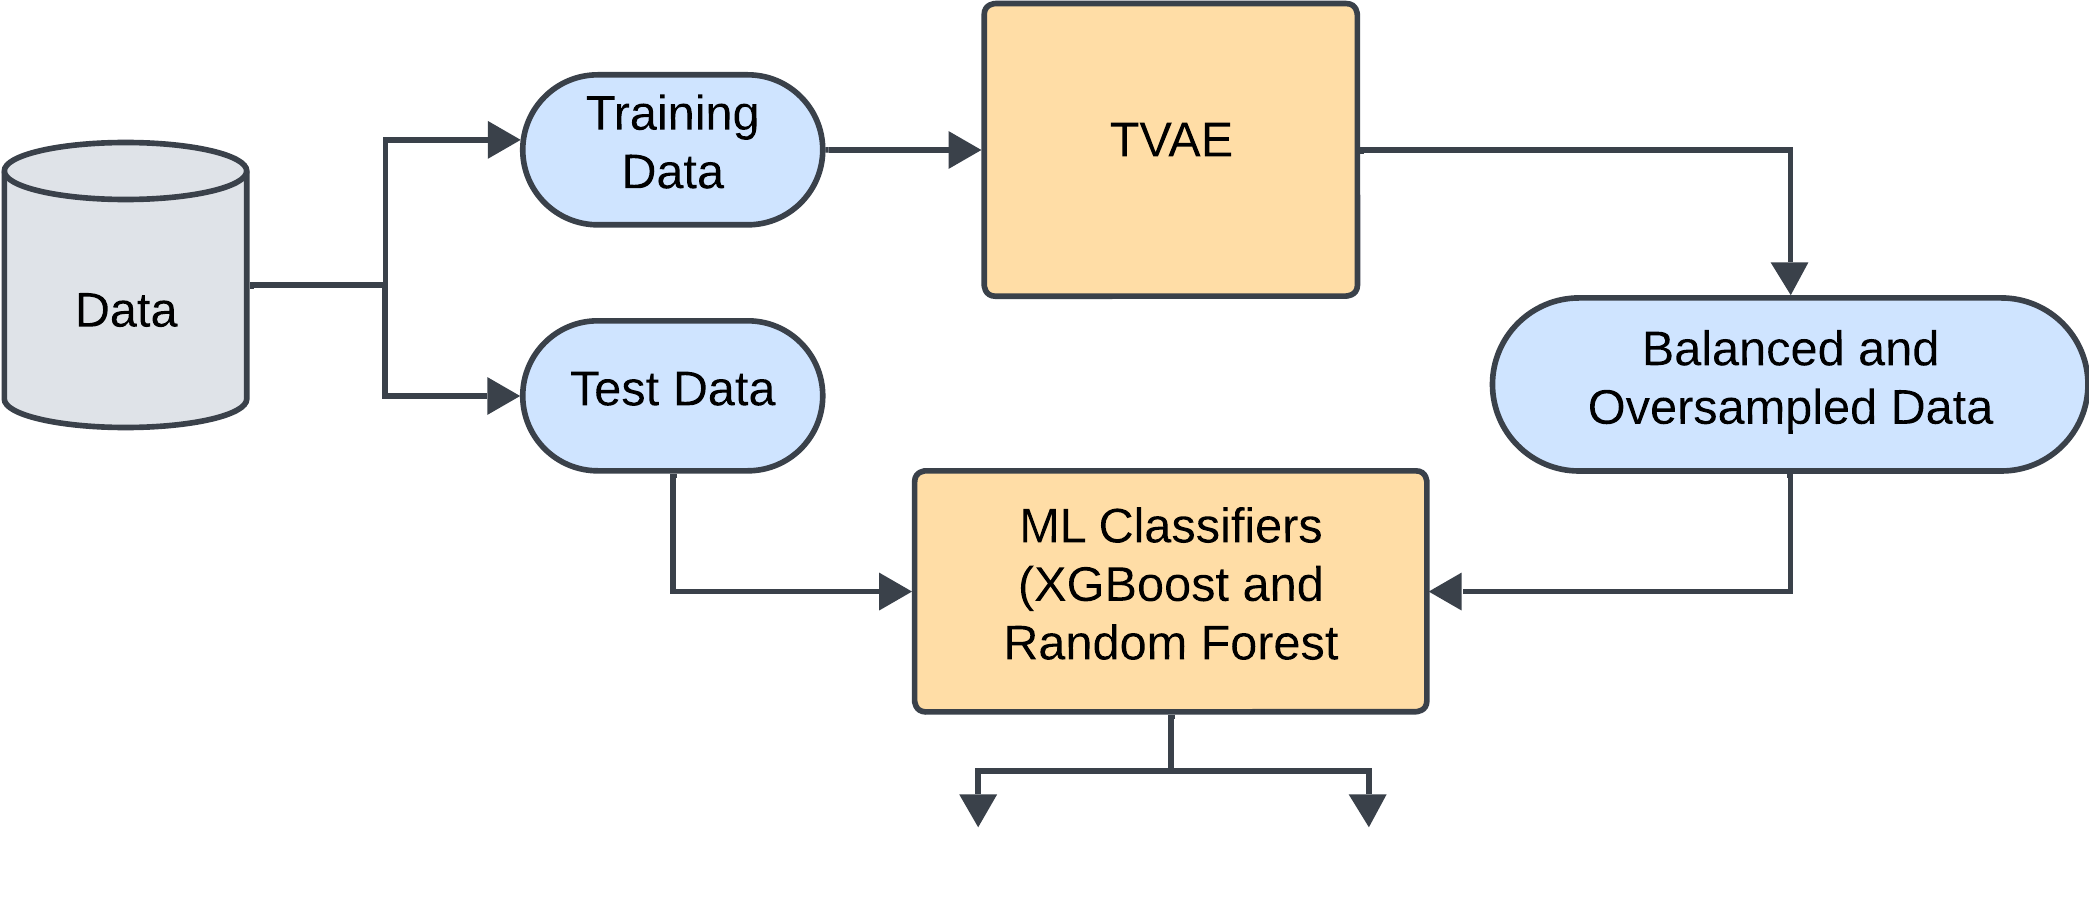
\includegraphics[width=0.85\textwidth]{images/model_tvae.png}
  \caption{Block diagram of the proposed approach to balance the training data and oversample both the classes using synthetic data generated using TVAE}
  \label{fig:model}
\end{figure}

\subsection{Tabular Variational Autoencoder (TVAE)}



\subsection{Data Preprocessing}
Before the data is fed to the machine learning models it need to be processed into format that can be easily understood and interpreted by the models. The TVAE implementation by SDV does not require any data preprocessing to be done from our side. The model does its own encoding and normalization depending on the type of features. In order to determine the type of features, SDV library requires us to pass the metedata of ous data in the form of JSON. As we are using decision tree ensemble models like XGBoost and Random Forest, we do not need to normalize or standardize the data, but we need to encode the features. Therefore, all the nominal features (As mentioned in Table \ref{tab:dataCols}) were one-hot encoded and all the ordinal features were label encoded.

\section{Results and Analysis}  \label{sec:result}
\subsection{Metrics}

\subsection{Evaluation}

\subsection{Results}

\begin{longtable}{|p{1.2cm}|p{1.2cm}|p{2.2cm}|p{2.3cm}|p{2.6cm}|p{2.2cm}|p{2cm}|p{2.2cm}|p{2.6cm}|}
\hline
\textbf{Work} & \textbf{Dataset} & \textbf{Methods} & \textbf{Balance Techniques} & \textbf{Order(Split/Balance)} & \textbf{Result Accuracy} & \textbf{Result Precision} & \textbf{Result Recall} & \textbf{Result F1-score} \\
\hline
[6] & carclaims.txt & ELM & Not Mentioned & Balance the data then split & 74.9\% & 74.9\% & 74.9\% & 74.9\% \\
\hline
[2] & carclaims.txt & Random Forest & SMOTE & Balance the data then split & 94.3\%, 98.6\%, 45.1\% & 94.3\%, 98.6\%, 45.1\% & 94.3\%, 98.6\%, 45.1\% & 94.3\%, 98.6\%, 45.1\%, 61.9\% \\
\hline
[3] & carclaims.txt & Random Forest & SMOTE \newline ROSE & Split Data then balance & 64.3\% \newline 61.34\% & -- \newline 14.1\% & 93.07\% \newline 95.24\% & 23.8\% \newline 22.79\% \\
\hline
[1] & carclaims.txt & Ensemble of SVM, MLP, KNN & FCM (Under Sampling), SMOTE & Balance the data then split & 81.2\% & -- & -- & 94.2\% \\
\hline
[5] & carclaims.txt & 4-layer 1D-CNN & SMOTE \newline CTGAN & Split Data then balance & 81.3\% \newline 79.3\% & 13.6\% \newline 16.7\% & 39.8\% \newline 61.5\% & 20.3\% \newline 26.2\% \\
\hline
Proposed & carclaims.txt & Random Forest XGBoost & TVAE & Split Data then balance and oversample & 87.13\% & 28.66\% & 66.83\% & 87.13\%, 28.66\%, 66.83\%, 40.12\% \\
\hline
\end{longtable}


\subsubsection{Balance data after split}

\begin{figure}
  \centering
  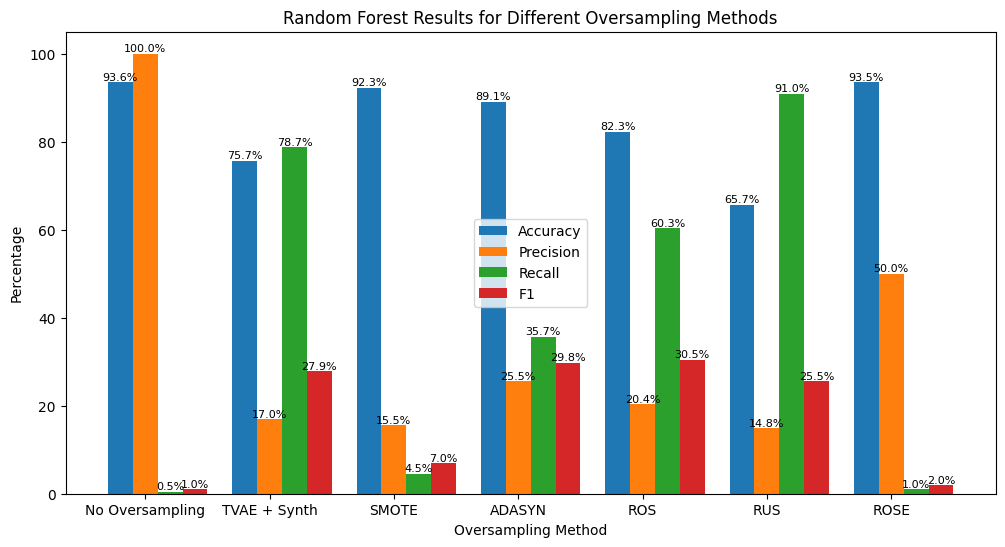
\includegraphics[width=0.85\textwidth]{images/rf_oversample_after_split.png}
  \caption{}
  \label{fig:rf_oversample_after_split}
\end{figure}

\begin{figure}
  \centering
  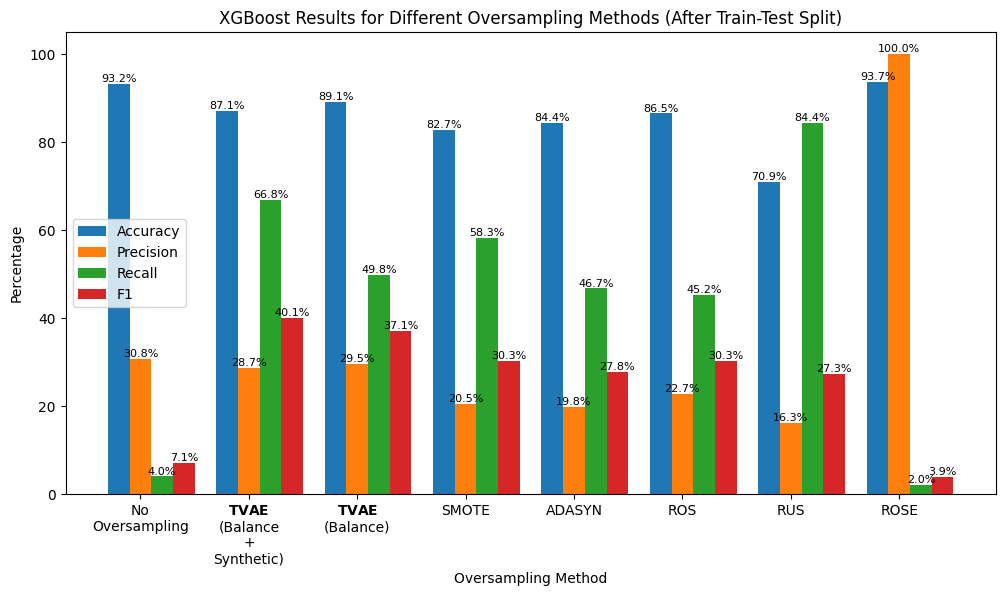
\includegraphics[width=0.85\textwidth]{images/xgboost_oversample_after_split.png}
  \caption{}
  \label{fig:xgboost_oversample_after_split}
\end{figure}

\subsubsection{Balance data before split}

\begin{figure}
  \centering
  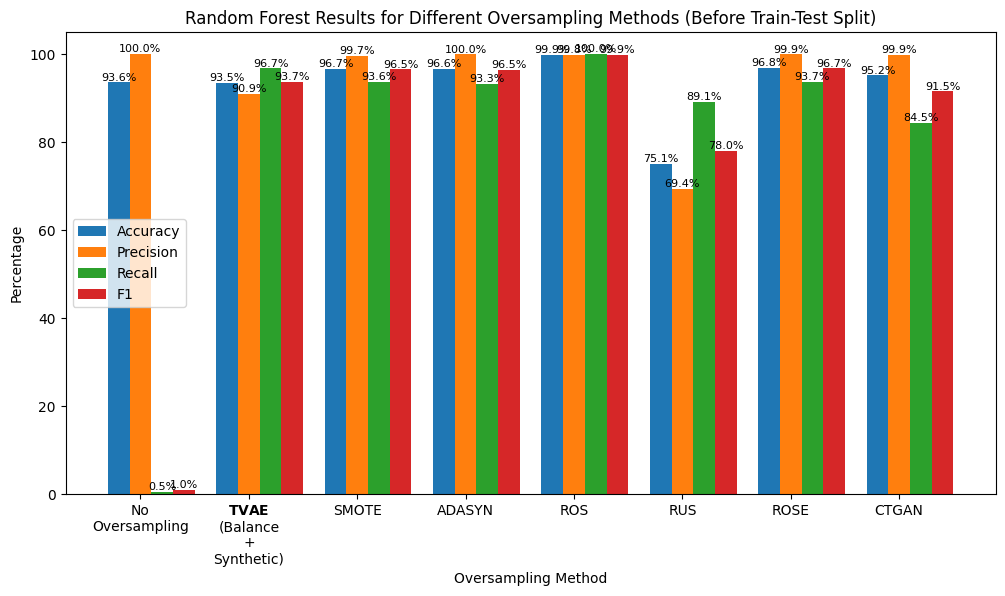
\includegraphics[width=0.85\textwidth]{images/rf_oversample_before_slit.png}
  \caption{}
  \label{fig:rf_oversample_after_split}
\end{figure}

\begin{figure}
  \centering
  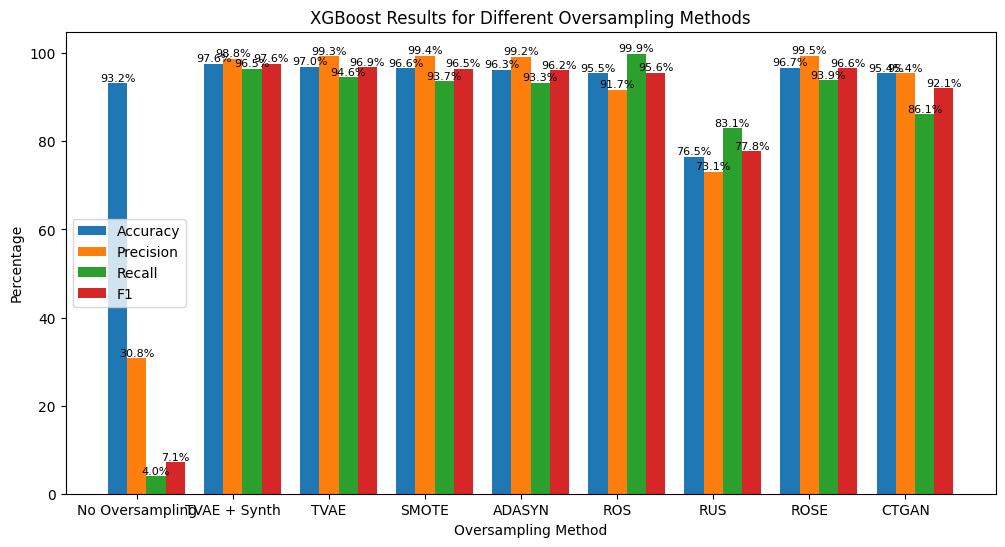
\includegraphics[width=0.85\textwidth]{images/xgboost_oversample_before_split.png}
  \caption{}
  \label{fig:xgboost_oversample_after_split}
\end{figure}

\section{Conclusion and Future Work}  \label{sec:conclusion}














% Acknowledgements and Disclosure of Funding should go at the end, before appendices and references

\acks{All acknowledgements go at the end of the paper before appendices and references.
Moreover, you are required to declare funding (financial activities supporting the
submitted work) and competing interests (related financial activities outside the submitted work).
More information about this disclosure can be found on the JMLR website.}


\appendix

\vskip 0.2in
\bibliography{references}

\end{document}
